% Rates of convergence of TD(lambda) in finite discounted MDPs.
% Numerics: experiments/td_lambda.py, experiments/figures_td.py, experiments/sweep.py
% Compile with:  tectonic td-lambda-rates.tex
\documentclass[11pt]{article}

\usepackage[T1]{fontenc}
\usepackage{lmodern}
\usepackage{amsmath,amssymb,amsthm}
\usepackage{mathtools}
\usepackage{booktabs}
\usepackage{graphicx}
\usepackage[margin=1.1in]{geometry}
\usepackage[colorlinks=true,linkcolor=blue,citecolor=blue,urlcolor=blue]{hyperref}
\emergencystretch=3em

\newtheorem{theorem}{Theorem}[section]
\newtheorem{lemma}[theorem]{Lemma}
\newtheorem{proposition}[theorem]{Proposition}
\newtheorem{corollary}[theorem]{Corollary}
\theoremstyle{definition}
\newtheorem{definition}[theorem]{Definition}
\newtheorem{assumption}[theorem]{Assumption}
\newtheorem{fact}[theorem]{Cited Fact}
\newtheorem{observation}[theorem]{Observation}
\theoremstyle{remark}
\newtheorem{remark}[theorem]{Remark}

\newcommand{\R}{\mathbb{R}}
\newcommand{\E}{\mathbb{E}}
\newcommand{\X}{\mathcal{S}}
\newcommand{\one}{\mathbf{1}}
\newcommand{\inner}[2]{\langle #1, #2\rangle}
\newcommand{\IV}{\mathrm{IV}}
\DeclareMathOperator{\tr}{tr}
\DeclareMathOperator{\spn}{span}

\title{Rates of Convergence of TD($\lambda$)\\ in Finite Discounted Markov Decision Processes}
\author{Vijaymohan Konda}
\date{November 2026}

\begin{document}
\maketitle

\begin{abstract}
For the evaluation of a fixed policy in a finite discounted MDP, we study how the
trace parameter $\lambda$ and the choice of features affect two quantities: the
quality of the TD($\lambda$) limit (its \emph{bias}) and the speed at which it is
reached (its \emph{intrinsic variance}, the asymptotic mean-squared error scaled by
the number of samples). Every quantity has a closed form for finite chains,
including the long-run noise covariance, which we compute exactly. The results are
organized as short statements with proofs; the few results we use without proof are
marked as \emph{cited facts}, and patterns supported only by computation are marked
as \emph{observations}. The main conclusions are: (i) the limit improves and the
signal strengthens as $\lambda$ increases, with explicit constants;
(ii) when the span of the features is invariant under the time-reversed chain, the
limit does not depend on $\lambda$ at all; (iii) the intrinsic variance depends only
on the span of the features, and recursive TD is never faster than least-squares TD;
(iv) contrary to what the bounds suggest, the intrinsic variance is \emph{not}
monotone in $\lambda$ in general, and can decrease along with the bias.
This chapter is the policy-evaluation layer of a study comparing actor-critic and
actor-only methods.
\end{abstract}

\tableofcontents

%======================================================================
\section{Setting}
%======================================================================

A fixed policy in a finite MDP induces a Markov reward process; we work with that
process directly.

\begin{assumption}[Standing assumptions]\label{ass:standing}
\begin{enumerate}
\item The state space $\X$ is finite, $P$ is a row-stochastic matrix on $\X$, and
  $g : \X \to \R$ is the expected one-stage reward under the policy.
\item $P$ is irreducible and aperiodic, with stationary distribution $\pi$; hence
  $\pi(x) > 0$ for all $x$. (For a strictly positive policy family this holds for
  every parameter as soon as it holds for one.)
\item The discount factor satisfies $\gamma \in [0,1)$, and $\lambda \in [0,1]$.
\item The feature matrix $\Phi \in \R^{\X \times m}$, with rows $\phi(x)^\top$, has
  linearly independent columns.
\item Samples are on-policy: $(x_k)$ is the Markov chain with transition matrix $P$,
  started from $\pi$.
\end{enumerate}
\end{assumption}

\paragraph{Notation.} $D = \operatorname{diag}(\pi)$,
$\inner{v}{w}_D = v^\top D w$, $\|v\|_D^2 = \inner{v}{v}_D$.
$\Pi = \Phi(\Phi^\top D\Phi)^{-1}\Phi^\top D$ is the $D$-orthogonal projection onto
$\spn\Phi$. $V = (I - \gamma P)^{-1} g$ is the value function.
$\tilde P(x,y) = \pi(y)P(y,x)/\pi(x)$ is the time-reversed chain, which is the
$D$-adjoint of $P$: $\inner{Pv}{w}_D = \inner{v}{\tilde Pw}_D$.
We write $c = \gamma\lambda$ and
\[
  K_\lambda = \gamma(1-\lambda)\, P\,(I - cP)^{-1}, \qquad
  \kappa_\lambda = \frac{\gamma(1-\lambda)}{1-\gamma\lambda} \in [0,\gamma].
\]
Note that $\kappa_0 = \gamma$, $\kappa_1 = 0$, and $\kappa_\lambda$ decreases in $\lambda$.

\paragraph{The algorithms.} With eligibility trace $z_k = c\, z_{k-1} + \phi(x_k)$
and temporal difference $d_k(r) = g(x_k) + \gamma\phi(x_{k+1})^\top r - \phi(x_k)^\top r$:
\begin{itemize}
\item \emph{recursive TD($\lambda$)}: $r_{k+1} = r_k + \alpha_k\, d_k(r_k)\, z_k$;
\item \emph{LSTD($\lambda$)}: $\hat r_n$ solves $\hat A_n \hat r_n + \hat b_n = 0$, where
  $\hat A_n = \frac1n\sum_{k<n} z_k(\gamma\phi(x_{k+1}) - \phi(x_k))^\top$ and
  $\hat b_n = \frac1n\sum_{k<n} z_k\, g(x_k)$.
\end{itemize}

%======================================================================
\section{The limit and its quality}
%======================================================================

Both algorithms target the solution of $A_\lambda r + b_\lambda = 0$, where
\[
  A_\lambda = \Phi^\top D (I - cP)^{-1}(\gamma P - I)\Phi, \qquad
  b_\lambda = \Phi^\top D (I - cP)^{-1} g .
\]

\begin{lemma}\label{lem:nonexp}
$\|Pv\|_D \le \|v\|_D$ for all $v$.
\end{lemma}
\begin{proof}
By Jensen's inequality and stationarity,
$\|Pv\|_D^2 = \sum_x \pi(x)\big(\sum_y P(x,y)v(y)\big)^2
\le \sum_x \pi(x)\sum_y P(x,y)v(y)^2 = \sum_y \pi(y) v(y)^2$.
\end{proof}

\begin{lemma}\label{lem:K}
$(I - cP)^{-1}(\gamma P - I) = K_\lambda - I$, and $\|K_\lambda v\|_D \le \kappa_\lambda\|v\|_D$.
\end{lemma}
\begin{proof}
Write $\gamma P - I = \gamma(1-\lambda)P - (I - cP)$ and multiply by $(I - cP)^{-1}$,
which commutes with $P$. For the bound, expand
$K_\lambda = \gamma(1-\lambda)\sum_{j\ge0} c^j P^{j+1}$ and use
Lemma~\ref{lem:nonexp}: $\|K_\lambda v\|_D \le \gamma(1-\lambda)\sum_j c^j\|v\|_D
= \kappa_\lambda\|v\|_D$.
\end{proof}

\begin{proposition}[Signal strength]\label{prop:signal}
For all $r \in \R^m$,
\[
  r^\top A_\lambda r \le -(1-\kappa_\lambda)\,\|\Phi r\|_D^2,
  \qquad 1 - \kappa_\lambda = \frac{1-\gamma}{1-\gamma\lambda}.
\]
In particular $A_\lambda$ is invertible and $r^*_\lambda = -A_\lambda^{-1}b_\lambda$ is
the unique limit. The constant $1-\kappa_\lambda$ increases from $1-\gamma$ at
$\lambda = 0$ to $1$ at $\lambda = 1$.
\end{proposition}
\begin{proof}
By Lemma~\ref{lem:K},
$r^\top A_\lambda r = \inner{\Phi r}{(K_\lambda - I)\Phi r}_D
\le \kappa_\lambda\|\Phi r\|_D^2 - \|\Phi r\|_D^2$ by Cauchy--Schwarz.
Since $\Phi$ has independent columns, $\|\Phi r\|_D > 0$ for $r \ne 0$.
\end{proof}

\begin{proposition}[Projected Bellman equation]\label{prop:projected}
Let $T_\lambda v = (I - cP)^{-1} g + K_\lambda v$. Then $V = T_\lambda V$, and
$\Phi r^*_\lambda$ is the unique fixed point in $\spn\Phi$ of $\Pi T_\lambda$.
\end{proposition}
\begin{proof}
$(I - cP)V = g + \gamma P V - cPV = g + \gamma(1-\lambda)PV$, so
$V = (I-cP)^{-1}g + K_\lambda V$. For the second claim,
$A_\lambda r + b_\lambda = \Phi^\top D\big(T_\lambda \Phi r - \Phi r\big)$ by
Lemma~\ref{lem:K}, and $\Phi^\top D w = 0$ means $\Pi w = 0$. So $A_\lambda r + b_\lambda = 0$
if and only if $\Pi T_\lambda\Phi r = \Phi r$. Uniqueness: $\Pi T_\lambda$ is a
$\kappa_\lambda$-contraction in $\|\cdot\|_D$, as $\Pi$ is nonexpansive.
\end{proof}

\begin{theorem}[Quality of the limit]\label{thm:bias}
\[
  \|\Phi r^*_\lambda - V\|_D \le \frac{\|\Pi V - V\|_D}{\sqrt{1-\kappa_\lambda^2}}.
\]
At $\lambda = 1$ the limit is the best approximation: $\Phi r^*_1 = \Pi V$.
\end{theorem}
\begin{proof}
Since $\Phi r^*_\lambda - \Pi V \in \spn\Phi$ is $D$-orthogonal to $\Pi V - V$,
\[
  \|\Phi r^*_\lambda - V\|_D^2 = \|\Phi r^*_\lambda - \Pi V\|_D^2 + \|\Pi V - V\|_D^2 .
\]
By Proposition~\ref{prop:projected},
$\Phi r^*_\lambda - \Pi V = \Pi T_\lambda\Phi r^*_\lambda - \Pi T_\lambda V
= \Pi K_\lambda(\Phi r^*_\lambda - V)$, whose norm is at most
$\kappa_\lambda\|\Phi r^*_\lambda - V\|_D$. Rearranging gives the bound; $\kappa_1 = 0$
gives the last claim.
\end{proof}

\begin{proposition}[Invariant subspaces remove the $\lambda$-dependence]\label{prop:invariant}
If $\tilde P(\spn\Phi) \subseteq \spn\Phi$, then $\Phi r^*_\lambda = \Pi V$ for every
$\lambda \in [0,1]$.
\end{proposition}
\begin{proof}
The $D$-adjoint of $K_\lambda$ is
$K_\lambda^* = \gamma(1-\lambda)\sum_j c^j\tilde P^{j+1}$, which maps $\spn\Phi$ into
itself. Hence for $u \in \spn\Phi$ and $w$ $D$-orthogonal to $\spn\Phi$,
$\inner{u}{K_\lambda w}_D = \inner{K^*_\lambda u}{w}_D = 0$, i.e.\ $\Pi K_\lambda(I-\Pi) = 0$.
Then
$\Pi T_\lambda(\Pi V) = \Pi T_\lambda V - \Pi K_\lambda(I-\Pi)V = \Pi V$, using
$V = T_\lambda V$. By uniqueness (Proposition~\ref{prop:projected}),
$\Phi r^*_\lambda = \Pi V$.
\end{proof}

\begin{remark}
The hypothesis holds when $\spn\Phi$ is spanned by eigenvectors of $\tilde P$, for
example Fourier features on a random walk on a cycle (circulant $P$), which is
example (b) below. Then the bias--variance trade-off in $\lambda$ disappears and only
the variance matters.
\end{remark}

%======================================================================
\section{Rates: intrinsic variance}
%======================================================================

Let $(x_k)_{k\in\mathbb{Z}}$ be the stationary two-sided chain, $z_k = \sum_{i\ge0}c^i\phi(x_{k-i})$
the stationary trace (the series converges because $c = \gamma\lambda \le \gamma < 1$), and
\[
  f_k = d_k(r^*_\lambda)\, z_k
\]
the noise at the limit. A trace started at time $0$ differs from $z_k$ by
$c^k z_{-1}$, which does not affect any of the asymptotic statements below.

\begin{fact}[Markov chain CLT]\label{fact:clt}
Under Assumption~\ref{ass:standing}, $\E f_k = 0$ (Lemma~\ref{lem:mean}),
the series $\Gamma = \sum_{l\in\mathbb{Z}}\E[f_0 f_l^\top]$ converges absolutely, and
$\frac1{\sqrt n}\sum_{k<n} f_k$ converges in distribution to $N(0,\Gamma)$.
Moreover $\hat A_n \to A_\lambda$ almost surely.
(Konda 2002, Thm.~6.1, whose conditions are verified for TD in Tsitsiklis and Van Roy
1997; see also Meyn and Tweedie, Ch.~17. Here $f_k$ is a bounded function of the past
of a finite, irreducible, aperiodic chain, and its dependence on the distant past
decays geometrically because the trace forgets at rate $c$.)
\end{fact}

\begin{theorem}[Rate of LSTD($\lambda$)]\label{thm:lstd}
$\sqrt n(\hat r_n - r^*_\lambda)$ converges in distribution to $N(0,\Sigma_0)$ with
$\Sigma_0 = A_\lambda^{-1}\Gamma A_\lambda^{-\top}$. Consequently $n\|\Phi(\hat r_n - r^*_\lambda)\|_D^2$ converges in distribution to a
random variable with mean equal to the \emph{intrinsic variance}
\[
  \IV(\lambda) = \tr\!\big(\Sigma_0\,\Phi^\top D\Phi\big).
\]
\end{theorem}
\begin{proof}
Since $z_k(g(x_k) + \gamma\phi(x_{k+1})^\top r^* - \phi(x_k)^\top r^*) = f_k$, we have
$\hat b_n + \hat A_n r^* = \frac1n\sum_{k<n} f_k$, hence exactly
\[
  \hat r_n - r^* = -\hat A_n^{-1}\Big(\frac1n\sum_{k<n} f_k\Big).
\]
Multiply by $\sqrt n$; by Fact~\ref{fact:clt} and Slutsky's lemma the limit is
$-A^{-1}N(0,\Gamma) = N(0, A^{-1}\Gamma A^{-\top})$. By the continuous mapping theorem
$n\|\Phi(\hat r_n - r^*)\|_D^2 \to \|\Phi w\|_D^2$ in distribution with
$w \sim N(0,\Sigma_0)$, and $\E\|\Phi w\|_D^2 = \tr(\Sigma_0\Phi^\top D\Phi)$.
\end{proof}

\begin{remark}
We use the mean of the limiting distribution rather than
$\lim_n n\,\E\|\Phi(\hat r_n - r^*)\|_D^2$, which can be infinite for finite $n$ when
$\hat A_n$ is singular with positive probability. In simulations the two agree.
\end{remark}

\begin{theorem}[Only the span of the features matters]\label{thm:basis}
Replace $\Phi$ by $\Phi B$ for an invertible $B \in \R^{m\times m}$. Then
$r^*$, $A$, $\Gamma$, $\Sigma_0$ become $B^{-1}r^*$, $B^\top AB$, $B^\top\Gamma B$,
$B^{-1}\Sigma_0B^{-\top}$. The LSTD approximations $\Phi\hat r_n$ are unchanged
sample path by sample path, and so are $\Phi r^*_\lambda$ and $\IV(\lambda)$.
\end{theorem}
\begin{proof}
Traces and features transform as $z \mapsto B^\top z$, $\phi \mapsto B^\top\phi$, so
$\hat A_n \mapsto B^\top\hat A_n B$ and $\hat b_n \mapsto B^\top\hat b_n$, and the
solution of the new system is $B^{-1}\hat r_n$; thus $\Phi B B^{-1}\hat r_n = \Phi\hat r_n$.
The same computation applies to $A, b, r^*$. The noise becomes $B^\top f_k$, so
$\Gamma \mapsto B^\top\Gamma B$, and $\Sigma_0 \mapsto B^{-1}A^{-1}B^{-\top}B^\top\Gamma B B^{-1}A^{-\top}B^{-\top}$.
Finally $\tr(B^{-1}\Sigma_0B^{-\top}B^\top\Phi^\top D\Phi B) = \tr(\Sigma_0\Phi^\top D\Phi)$.
\end{proof}

\subsection{Recursive TD is never faster than LSTD}

\begin{fact}[Rate of recursive TD]\label{fact:td}
With steps $\alpha_k = \alpha/k$ and $K = \alpha A_\lambda + \tfrac12 I$ Hurwitz,
$\sqrt k(r_k - r^*)$ is asymptotically $N(0,\Sigma_{\mathrm{TD}})$, where
$K\Sigma_{\mathrm{TD}} + \Sigma_{\mathrm{TD}}K^\top + \alpha^2\Gamma = 0$.
(Konda 2002, Thm.~6.1; Benveniste, M\'etivier and Priouret, Thm.~13, p.~332.)
\end{fact}

\begin{lemma}[Lyapunov equations]\label{lem:lyap}
If $K$ is Hurwitz and $KX + XK^\top = -Q$ with $Q \succeq 0$, then
$X = \int_0^\infty e^{Kt}Qe^{K^\top t}\,dt \succeq 0$.
\end{lemma}
\begin{proof}
$\frac{d}{dt}\big(e^{Kt}Xe^{K^\top t}\big) = e^{Kt}(KX + XK^\top)e^{K^\top t}
= -e^{Kt}Qe^{K^\top t}$. Integrate over $[0,\infty)$ and use $e^{Kt}\to0$.
\end{proof}

\begin{theorem}[TD versus LSTD]\label{thm:td-lstd}
Under the conditions of Fact~\ref{fact:td},
\[
  \Sigma_{\mathrm{TD}} - \Sigma_0 \succeq 0,
\]
with equality if and only if $(\alpha I + A_\lambda^{-1})\Gamma = 0$; when $\Gamma \succ 0$,
if and only if $A_\lambda = -\alpha^{-1}I$.
\end{theorem}
\begin{proof}
Write $A = A_\lambda$ and $X = \Sigma_{\mathrm{TD}} - \Sigma_0$. From
$\Sigma_0 = A^{-1}\Gamma A^{-\top}$ we get
$K\Sigma_0 + \Sigma_0K^\top = \alpha(\Gamma A^{-\top} + A^{-1}\Gamma) + \Sigma_0$. Hence
\[
  KX + XK^\top = -\alpha^2\Gamma - \alpha\Gamma A^{-\top} - \alpha A^{-1}\Gamma - A^{-1}\Gamma A^{-\top}
  = -(\alpha I + A^{-1})\,\Gamma\,(\alpha I + A^{-1})^\top ,
\]
and Lemma~\ref{lem:lyap} gives $X \succeq 0$. The integrand vanishes identically iff
$(\alpha I + A^{-1})\Gamma(\alpha I + A^{-1})^\top = 0$, iff
$(\alpha I + A^{-1})\Gamma^{1/2} = 0$.
\end{proof}

\begin{remark}
Equality needs $A_\lambda$ to be a negative multiple of the identity, hence symmetric.
For $\lambda = 1$, $A_1 = -\Phi^\top D\Phi$ is symmetric, so TD(1) with $\alpha = 1$
and $D$-orthonormal features is as fast as LSTD(1). For $\lambda < 1$, $A_\lambda$ is
generally not symmetric, and since a change of basis maps $A$ to $B^\top AB$, which
preserves (non)symmetry, recursive TD($\lambda$) is then, when $\Gamma \succ 0$, strictly
slower than LSTD($\lambda$) in every basis and for every $\alpha$. (Polyak--Ruppert averaging of
the recursive iterates recovers $\Sigma_0$; Konda 2002, Sec.~6.2.1.)
\end{remark}

%======================================================================
\section{Exact computation of the noise covariance}
%======================================================================

We now give $\Gamma$ in closed form. Let $r = r^*_\lambda$ and define
\begin{align*}
  d(x,y) &= g(x) + \gamma\phi(y)^\top r - \phi(x)^\top r, &
  \bar d(x) &= \textstyle\sum_y P(x,y)d(x,y), \\
  u &= (I - cP)^{-1}\bar d \in \R^\X, &
  W(x) &= \phi(x)\,u(x) \in \R^m, \\
  \mu &= (I - c\tilde P)^{-1}\Phi, &
  \mu^-(x) &= \textstyle\sum_y\tilde P(x,y)\mu(y),
\end{align*}
and let $q = \sum_{n\ge1}P^nW = (Z - I)W$ with $Z = (I - P + \one\pi^\top)^{-1}$
(convergence is shown in Lemma~\ref{lem:mean}). Let $M : \X \to \R^{m\times m}$ be the
solution of the linear system
\[
  M(x) = \phi(x)\phi(x)^\top + c\big(\phi(x)\mu^-(x)^\top + \mu^-(x)\phi(x)^\top\big)
    + c^2\sum_y\tilde P(x,y)M(y),
\]
which is unique since $c^2 < 1$.

\begin{lemma}[Moments of the stationary trace]\label{lem:trace}
$\E[z_0 \mid x_0] = \mu(x_0)$, $\E[z_{-1}\mid x_0] = \mu^-(x_0)$ and
$\E[z_0z_0^\top\mid x_0] = M(x_0)$. Moreover, given $x_0$, the trace $z_0$ is independent
of $(x_1, x_2, \dots)$.
\end{lemma}
\begin{proof}
Run backwards in time, $(x_0, x_{-1}, x_{-2},\dots)$ is a Markov chain with transition
matrix $\tilde P$, so $\E[\phi(x_{-i})\mid x_0] = (\tilde P^i\Phi)(x_0)$ and
$\E[z_0\mid x_0] = \sum_i c^i(\tilde P^i\Phi)(x_0) = \mu(x_0)$; then
$\E[z_{-1}\mid x_0] = \E[\E[z_{-1}\mid x_{-1}]\mid x_0] = (\tilde P\mu)(x_0)$.
For the second moment, $z_0 = \phi(x_0) + c z_{-1}$, so
$\E[z_0z_0^\top\mid x_0]$ equals
$\phi\phi^\top + c(\phi\,\mu^{-\top} + \mu^-\phi^\top) + c^2\E[z_{-1}z_{-1}^\top\mid x_0]$,
and by the backward Markov property the last term is
$\sum_y\tilde P(x_0,y)\E[z_{-1}z_{-1}^\top\mid x_{-1} = y]$. Stationarity makes the
conditional second moment the same function $M$ at every time. The independence
claim is the Markov property: $z_0$ is a function of the past.
\end{proof}

\begin{lemma}[Mean of the noise]\label{lem:mean}
$\E f_0 = \Phi^\top Du = \pi^\top W$, and this equals $A_\lambda r + b_\lambda = 0$.
Consequently $\|P^nW\| \to 0$ geometrically and $q$ is well defined.
\end{lemma}
\begin{proof}
$\E f_0 = \sum_i c^i\E[\phi(x_{-i})\bar d(x_0)] = \sum_i c^i\Phi^\top DP^i\bar d
= \Phi^\top Du$, using $\E[\phi(x_{-i})h(x_0)] = \Phi^\top DP^ih$. Since
$\bar d = g + (\gamma P - I)\Phi r$, this is $b_\lambda + A_\lambda r = 0$. By aperiodicity
and irreducibility $P^n \to \one\pi^\top$ geometrically, so
$P^nW \to \one\,\pi^\top W = 0$ geometrically; then
$\sum_{n\ge0}P^nW = \sum_{n\ge0}(P - \one\pi^\top)^nW = ZW$.
\end{proof}

\begin{lemma}[Accumulated future noise]\label{lem:future}
Let $\mathcal F_1 = \sigma(x_j : j \le 1)$. As $L\to\infty$,
\[
  \sum_{l=1}^L\E[f_l\mid\mathcal F_1] \longrightarrow u(x_1)\,z_1 + q(x_1) - \beta
\]
boundedly and almost surely, for a deterministic vector $\beta \in \R^m$.
\end{lemma}
\begin{proof}
For $l\ge1$, $\E[f_l\mid\mathcal F_l] = \bar d(x_l)z_l$, and
$z_l = c^{l-1}z_1 + \sum_{j=2}^lc^{l-j}\phi(x_j)$. Taking $\E[\cdot\mid\mathcal F_1]$ and
summing,
\[
  \sum_{l=1}^L\E[f_l\mid\mathcal F_1]
  = \Big(\sum_{l=1}^Lc^{l-1}(P^{l-1}\bar d)(x_1)\Big)z_1
    + \sum_{j=2}^{L}\big(P^{j-1}[\Phi\odot u_{L-j}]\big)(x_1),
\]
where $u_N = \sum_{i=0}^Nc^iP^i\bar d$ and $(\Phi\odot v)(x) = \phi(x)v(x)$. The first
term tends to $u(x_1)z_1$. Write $u_N = u - t_N$ with $\|t_N\|_\infty \le Cc^N$. The part with
$u$ tends to $q(x_1)$ by Lemma~\ref{lem:mean}. For the tail part, write
$P^{j-1} = \one\pi^\top + (P^{j-1} - \one\pi^\top)$ with
$\|P^{j-1} - \one\pi^\top\|_\infty\le C\rho^{j-1}$ for some $\rho<1$, and set $N = L - j$:
\[
  \sum_{j=2}^L P^{j-1}[\Phi\odot t_{L-j}]
  = \one\sum_{N=0}^{L-2}\pi^\top[\Phi\odot t_N] + O\Big(\sum_{N=0}^{L-2}\rho^{L-N-1}c^N\Big).
\]
The first sum converges absolutely to some $\beta$, and the error term tends to zero.
All quantities are bounded uniformly in $L$ because $\Phi$, $\bar d$ and $z$ are bounded.
\end{proof}

\begin{theorem}[Closed form for $\Gamma$]\label{thm:gamma}
$\Gamma = E_0 + T + T^\top$, where
\begin{align*}
  E_0 &= \sum_{x,y}\pi(x)P(x,y)\,d(x,y)^2\,M(x), \\
  T &= \sum_{x,y}\pi(x)P(x,y)\,d(x,y)\Big[u(y)\big(c\,M(x) + \mu(x)\phi(y)^\top\big) + \mu(x)\,q(y)^\top\Big].
\end{align*}
\end{theorem}
\begin{proof}
$E_0 = \E[f_0f_0^\top] = \E[d(x_0,x_1)^2\,\E[z_0z_0^\top\mid x_0,x_1]]$, and by
Lemma~\ref{lem:trace} the inner expectation is $M(x_0)$. For the off-diagonal part,
$f_0$ is $\mathcal F_1$-measurable, so by Lemma~\ref{lem:future} and bounded
convergence,
\[
  T = \sum_{l\ge1}\E[f_0f_l^\top] = \lim_L\E\Big[f_0\Big(\sum_{l=1}^L\E[f_l\mid\mathcal F_1]\Big)^\top\Big]
  = \E\big[f_0\big(u(x_1)z_1 + q(x_1)\big)^\top\big] - \E[f_0]\beta^\top ,
\]
and the last term vanishes by Lemma~\ref{lem:mean}. Substitute
$z_1 = cz_0 + \phi(x_1)$ and use Lemma~\ref{lem:trace}:
$\E[z_0z_1^\top\mid x_0,x_1] = cM(x_0) + \mu(x_0)\phi(x_1)^\top$ and
$\E[z_0\mid x_0,x_1] = \mu(x_0)$. Finally, $\sum_{l\le -1}\E[f_0f_l^\top] = T^\top$ by
stationarity.
\end{proof}

\begin{remark}[Numerical check]
Theorem~\ref{thm:gamma} is implemented in \texttt{experiments/td\_lambda.py}. On the
two test chains below, Monte Carlo estimates of $n\,\E\|\Phi(\hat r_n - r^*)\|_D^2$
(4000 runs of length 4000) agree with $\IV(\lambda)$ to within 2\%, the Monte Carlo
error, for $\lambda \in \{0, 0.5, 0.9\}$; and $\IV$ is unchanged to six digits under
random changes of basis, as Theorem~\ref{thm:basis} predicts.
\end{remark}

%======================================================================
\section{The trade-off in $\lambda$}
%======================================================================

\begin{definition}
The \emph{asymptotic error proxy} after $n$ samples is
$\mathcal E_n(\lambda) = \|\Phi r^*_\lambda - V\|_D^2 + \IV(\lambda)/n$, the leading terms of
$\E\|\Phi\hat r_n - V\|_D^2$; and $\lambda^*(n)$ denotes a minimizer.
\end{definition}

The bounds of Section~2 and Konda (2002, Sec.~6.2.2) suggest the classical picture:
the bias decreases in $\lambda$ while the variance increases, so $\lambda^*(n)$ increases
from small values towards $1$ as $n$ grows. The computations show that the bias half
of this picture is robust, but the variance half is not.

\begin{figure}[t]
\centering
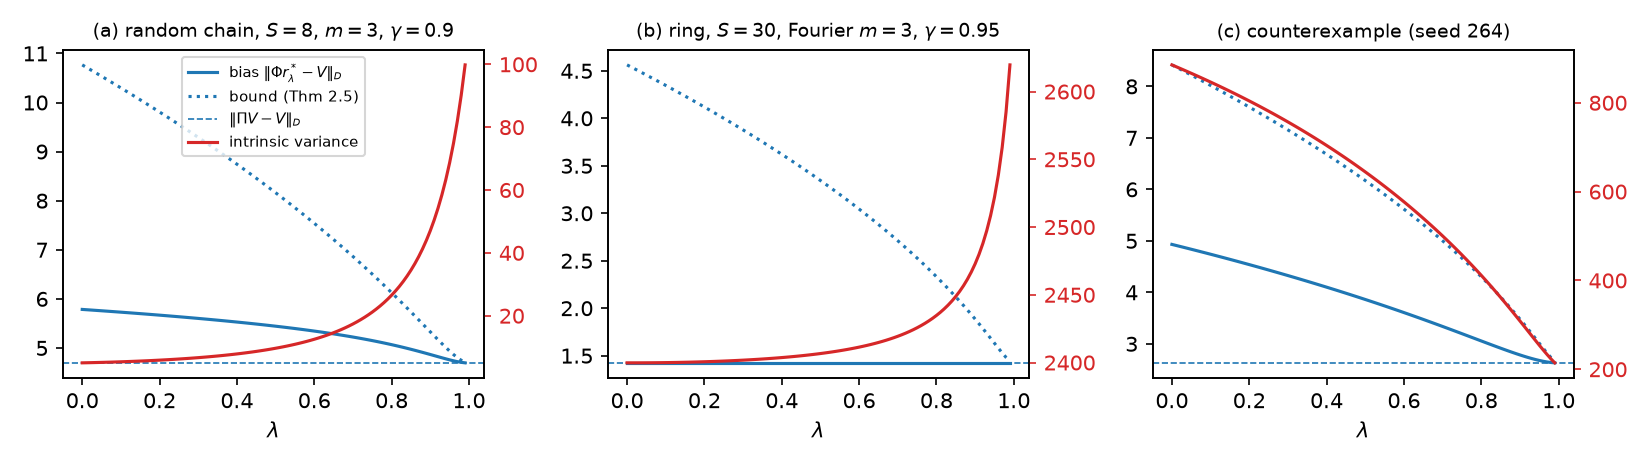
\includegraphics[width=\textwidth]{figures/td_bias_variance.png}
\caption{Bias (blue, left axis), the bound of Theorem~\ref{thm:bias} (dotted), the
best possible error $\|\Pi V - V\|_D$ (dashed), and intrinsic variance (red, right axis)
as functions of $\lambda$. (a) a random chain; (b) a slowly mixing ring with Fourier
features, where Proposition~\ref{prop:invariant} applies and the bias is flat;
(c) a chain where the intrinsic variance \emph{decreases} with $\lambda$.}
\label{fig:bv}
\end{figure}

\begin{observation}[Typical behaviour]\label{obs:typical}
For the random chain of Figure~\ref{fig:bv}(a)
($|\X| = 8$, $m = 3$, $\gamma = 0.9$), the intrinsic variance grows twentyfold, from
$5.0$ at $\lambda = 0$ to $99.8$ at $\lambda = 0.99$, while the bias falls from $5.78$ to
$4.70$ (the best possible is $4.69$). Recursive TD with the best constant $\alpha$ has
about twice the intrinsic variance of LSTD at every $\lambda$
(e.g.\ $19.4$ versus $9.6$ at $\lambda = 0.5$).
\end{observation}

\begin{observation}[Frequency of the patterns]\label{obs:sweep}
Over 300 random chains ($5 \le |\X| \le 14$, $1 \le m \le 4$, $\gamma \in \{0.8, 0.9, 0.95\}$,
$\lambda$ on a grid of 34 values in $[0,0.99]$):
\begin{itemize}
\item TD $\ge$ LSTD held in all 300 cases, as Theorem~\ref{thm:td-lstd} requires; the
  ratio of intrinsic variances at $\lambda = 0.3$ had median $1.26$ and maximum $17.2$.
\item $\IV(\lambda)$ was monotone increasing in 269 cases and \emph{not} monotone in 31;
  in one case (Figure~\ref{fig:bv}(c)) it decreased by $76\%$ from its maximum to
  $\lambda = 0.99$, so that $\lambda \to 1$ is best for every $n$.
\item The bias was monotone decreasing in 269 cases; in the other 31 the largest
  increase along $\lambda$ was at most $1.2\%$ of the bias at $\lambda = 0$ (median $0.05\%$).
\item In 281 cases, $\lambda^*(n)$ lay strictly inside $(0,1)$ for some
  $n \in \{10, 10^2, 10^3, 10^4\}$, so the trade-off is genuine in most instances.
\end{itemize}
\end{observation}

\begin{figure}[t]
\centering
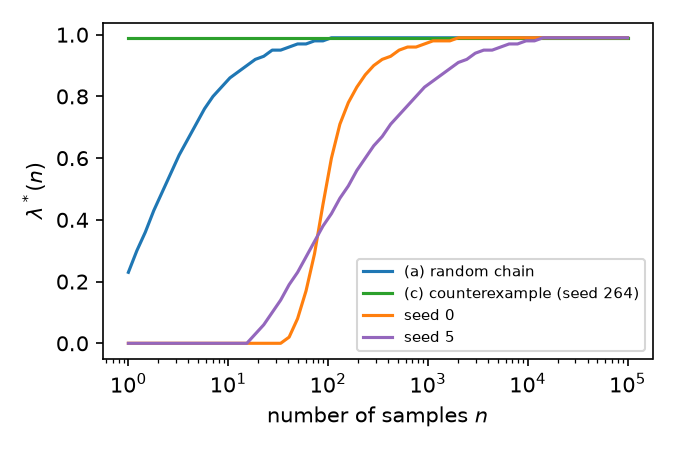
\includegraphics[width=0.55\textwidth]{figures/td_best_lambda.png}
\caption{The best trace parameter $\lambda^*(n)$ as a function of the number of samples,
for four chains. It moves from small values to $1$ as $n$ grows, at a rate set by the
ratio of the bias gap to the variance gap; for the chain of Figure~\ref{fig:bv}(c) it
equals $1$ throughout.}
\label{fig:best}
\end{figure}

\begin{observation}[Features]\label{obs:features}
On the ring of Figure~\ref{fig:bv}(b) with nested Fourier bases of size
$m = 1, 3, 5, 7, 9, 15$ and $\lambda = 0.5$, the bias decreases
($10.58, 1.42, 0.40, 0.39, 0.37, 0.19$), but the intrinsic variance is not monotone:
$7065$ for $m = 1$, then $2407, 2618, 2838, 2947, 3033$. Enlarging the span can thus
lower both bias and variance, or trade one for the other.
\end{observation}

%======================================================================
\section{Summary and next step}
%======================================================================

\begin{itemize}
\item \emph{Proved.} Larger $\lambda$ strengthens the signal
  (Proposition~\ref{prop:signal}) and improves the guaranteed quality of the limit
  (Theorem~\ref{thm:bias}); with invariant feature spans, $\lambda$ does not affect the
  limit at all (Proposition~\ref{prop:invariant}). The rate depends only on the span of the
  features (Theorem~\ref{thm:basis}), recursive TD is never faster than LSTD, and for
  $\lambda < 1$ it is strictly slower in every basis (Theorem~\ref{thm:td-lstd}). The
  long-run noise covariance has a closed form (Theorem~\ref{thm:gamma}).
\item \emph{Observed.} The intrinsic variance usually increases with $\lambda$, but not
  always, and can fall together with the bias; the number of samples at which large
  $\lambda$ pays off varies widely between instances.
\end{itemize}

The next chapter uses the same machinery for the actor: the asymptotic covariance of
the actor's parameter in a two-time-scale actor-critic algorithm reduces to a
single-time-scale iteration (Konda 2002, Thm.~7.8), whose noise combines the actor's
own noise with the critic's noise $f_k$ studied here. That reduction lets us compare,
with exact numbers, actor-critic algorithms using TD($\lambda$) critics for
$\lambda < 1$ with actor-only methods, the case left open in Section~8.4 of the thesis.

\begin{thebibliography}{9}
\bibitem{konda2002}
V.~R. Konda. \emph{Actor-Critic Algorithms}. PhD thesis, MIT, 2002.
\bibitem{bmp}
A.~Benveniste, M.~M\'etivier and P.~Priouret. \emph{Adaptive Algorithms and
  Stochastic Approximations}. Springer, 1990.
\bibitem{mt}
S.~P. Meyn and R.~L. Tweedie. \emph{Markov Chains and Stochastic Stability}.
  Cambridge University Press, 2nd ed., 2009.
\bibitem{tvr}
J.~N. Tsitsiklis and B.~Van~Roy. An analysis of temporal-difference learning with
  function approximation. \emph{IEEE Trans.\ Automatic Control}, 42(5):674--690, 1997.
\end{thebibliography}

\end{document}
